%! Author = noone
%! Date = 8/10/22

% Preamble
\documentclass[11pt]{article}
\documentclass{beamer}
% Packages
\usepackage{amsmath}
\usepackage{graphicx}
\usepackage{hyperref}
\usepackage{float}
\usepackage{multimedia}
\usepackage{blindtext}

% Document
\begin{document}

\section{Long Short Term Memory}\label{sec:long-short-term-memory}

Simple Recurrent Networks (SRNs) can learn medium-range dependencies but have difficulty learning long range dependencies.
Long Short Term Memory (LSTM) is able to learn long range dependencies using a combination of forget, input and output gates (Hochreiter and Schmidhuber, 1998).

\begin{figure}[h]
    \centering
    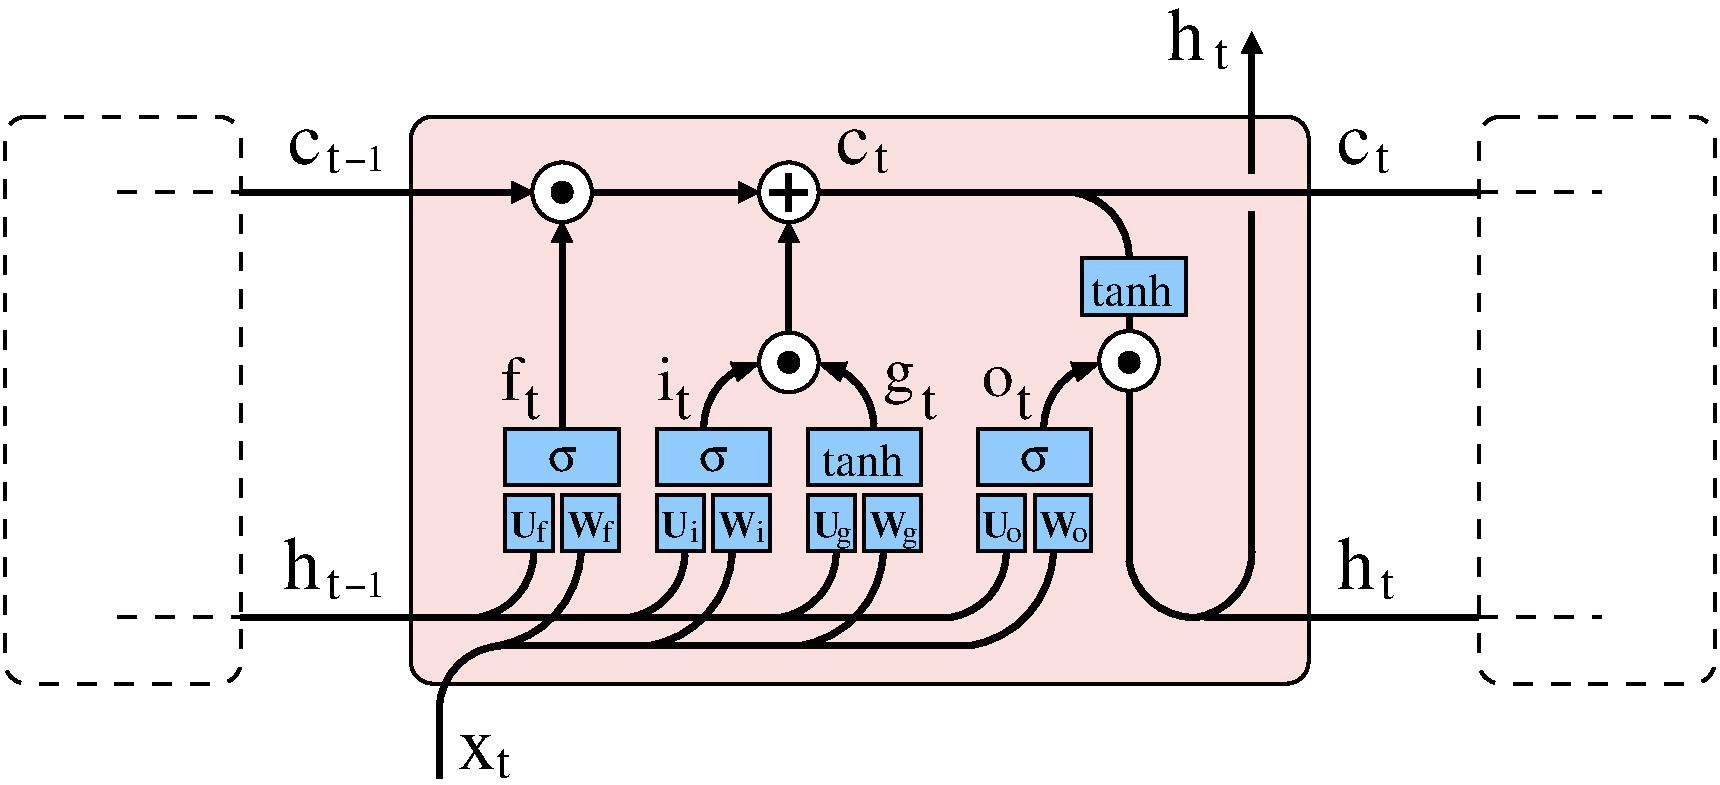
\includegraphics[width=12,height=8]{../out/images/lstm}
    \caption[LSTM]{LSTM}
    \label{fig: LSTM}
\end{figure}

The LSTM maintains a context layer which is distinct from the hidden layer but contains the same number of units.
The full workings of the LSTM at each timestep are described by these equations:

\textbf{Gates}

\begin{gather*}
    f_t = \sigma (U_f h_{t-1} + W_{f X_t} + b_f)\\
    i_t = \sigma(U_i h_{t-1} W_{i X_t} + b_i)\\
    o_i = \sigma(U_o h_{t-1} + W_{o X_t} + b_o)\\
\end{gather*}

\textbf{Candidate activation}

\[g_t = \tanh (U_g h_{t-1} + W_{g X_t})\]

\textbf{State}

\[c_t = f_t \odot c_{t-1} + i_t \odot g_t\]

\textbf{Outputs}:

\[h_t = o_t \odot \tanh c_t\]

First, the **forget** gate ($f$) is used to determine, for each context unit, a ratio between 0 and 1 by which the value of this context unit will be multiplied.
If the ratio is close to zero, the previous value of the corresponding context unit will be largely forgotten;
if it is close to 1, the previous value will be largely preserved.

Next, \textbf{update} values ($g$) between $-1$ and $+1$ are computed using $\tanh$, and the input gate ($i$) is used to determine ratios by which these update values will be multiplied before being added to the current context values.

Finally, the \textbf{output} gate ($o$) is computed and used to determine the ratios by which $\tanh$ of the context unit values will be multiplied in order to produce the next hidden unit values.

In this way, the context units are able to specialise, with some of them changing their values frequently while others preserve their state for many timesteps, until particular circumstances cause the gates to be opened and allow the value of those units to change.

\subsection{Embedded Reber Grammar}\label{subsec:embedded-reber-grammar}

The ability of different sequence processing algorithms to learn long range dependencies can be explored using the Reber Grammar and Embedded Reber Grammar.
\begin{figure}[h]
    \centering
    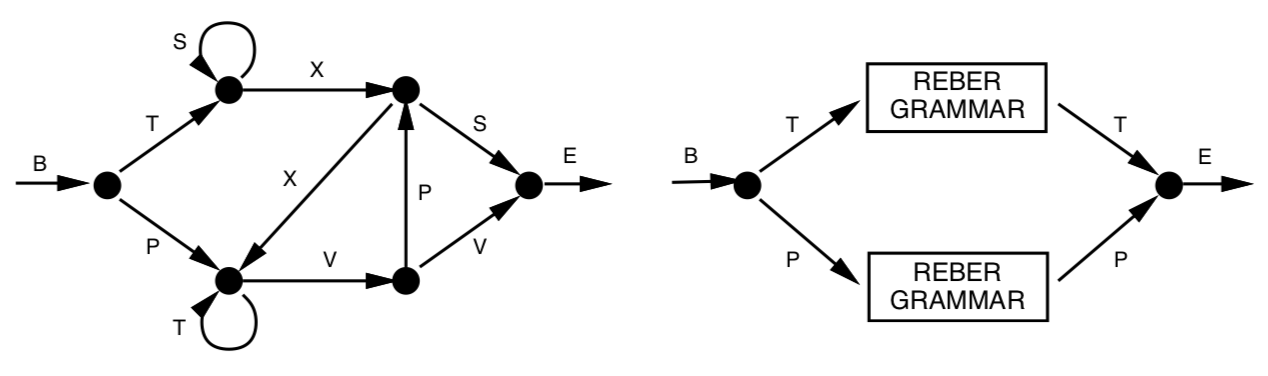
\includegraphics[width=12,height=4]{../out/images/reber-grammar}
    \caption[reber grammar]{reber grammar}
    \label{fig: reber grammar}
\end{figure}

The Reber Grammar (RG) is defined by the finite state machine shown on the left.
When there is a choice between two transitions, they are understood to be chosen with equal probability.
The Embedded Reber Grammar (ERG) is shown on the right, where each box marked \textbf{REBER GRAMMAR} contains an identical copy of the finite state machine on the left.
The difficulty in learning the ERG is that the network must remember which transition (T or P)  occurred after the initial B, and retain this information while it is processing the transitions associated with the RG in one of the two identical boxes, in order to correctly predict the T or P occurring before the final E.

In the exercises for this week, you will be demonstrating that the SRN is able to learn the RG but struggles to learn the ERG, whereas the LSTM can also learn the ERG. We can imagine that one of the context units is somehow assigned the task of retaining the knowledge of the initial T or P, and that this knowledge is preserved by appropriately high and low values for the forget gate and the input and output gate, respectively.

\subsection{Gated Recurrent Unit}\label{subsec:gated-recurrent-unit}

\begin{figure}[h]
    \centering
    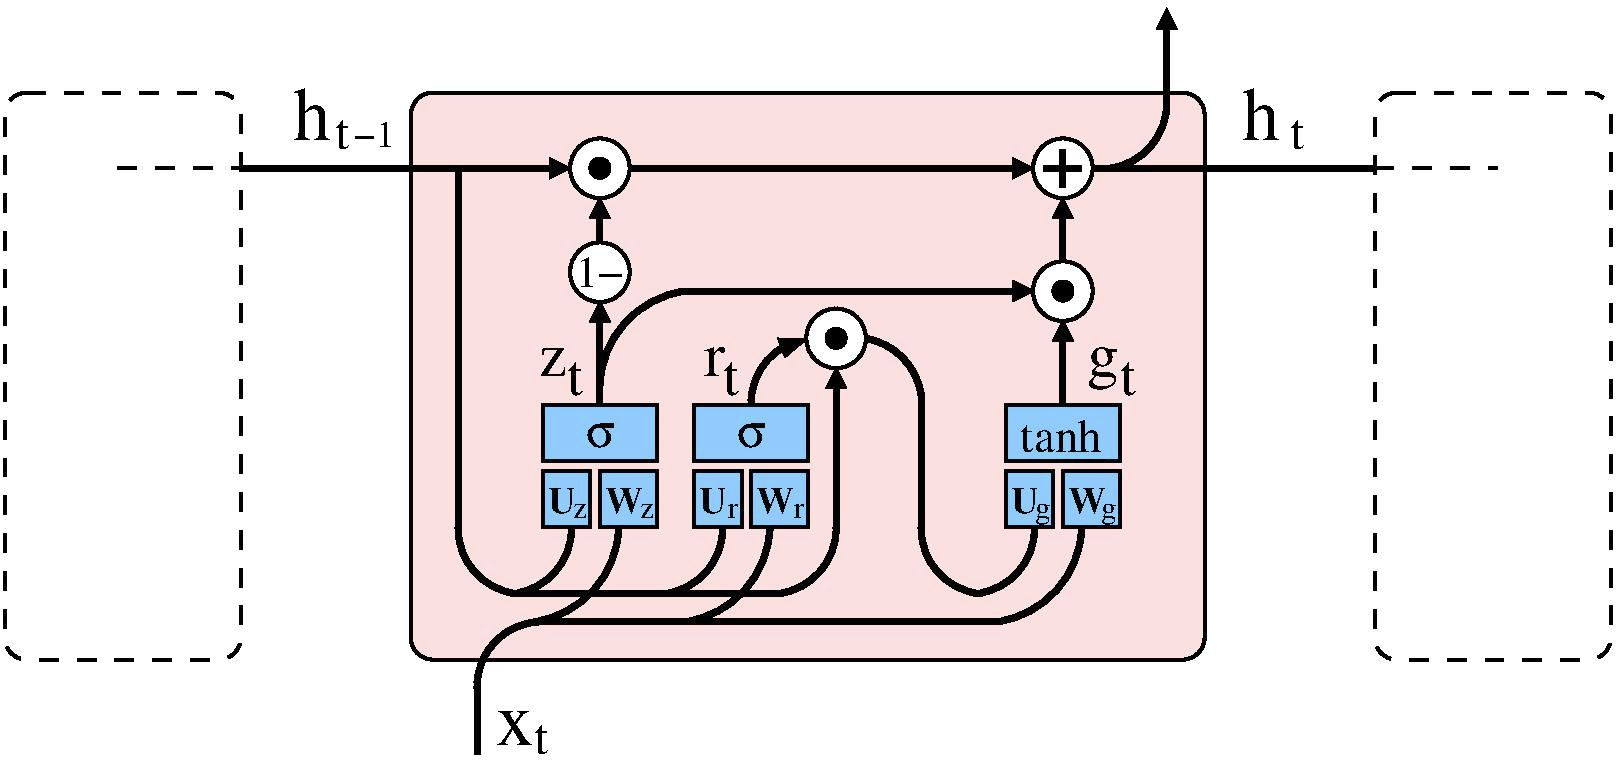
\includegraphics[height=6,width=12]{../out/images/gated-recurrent-unit}
    \caption[gated recurrent unit]{gated recurrent unit}
    \label{fig: gated recurrent unit}
\end{figure}

The Gated Recurrent Unit (GRU) is similar to LSTM but has only two gates instead of three.
Its update equations are as follows:

\textbf{Gates}

\begin{gather*}
    z_t = \sigma (U_{z}h_{t-1} + W_{z}X_t + b_z)\\
    r_t = \sigma (U_g(r_t \odot h_{t-1}) + W_g X_{t} + b_g)\\
\end{gather*}

\textbf{Candidate Activation}

\textbf{Output}

\subsection{Optional Video}\label{subsec:optional-video}

\subsection{further reading}\label{subsec:further-reading}

Fahlman, S. E. (1991). \href{https://citeseerx.ist.psu.edu/viewdoc/download?doi=10.1.1.52.7163&rep=rep1&type=pdf}{The recurrent cascade-correlation architecture} (Technical Report CMU-CS-91-100). Carnegie-Mellon University, Department of Computer Science.

Hochreiter, S., and Schmidhuber, J., 1997. \href{http://citeseerx.ist.psu.edu/viewdoc/download?doi=10.1.1.676.4320&rep=rep1&type=pdf}{Long short-term memory}. Neural Computation, 9(8), 1735-1780.

Two excellent web resources for LSTM:
- \href{http://colah.github.io/posts/2015-08-Understanding-LSTMs/}{Understanding LSTM Networks} (Colah, 2015. Github)
- \href{http://christianherta.de/lehre/dataScience/machineLearning/neuralNetworks/LSTM.php}{LSTM (Long Short Term Memory} (Huerta, n.d. christianherta.de)
- \href{https://www.deep-teaching.org/notebooks/sequence-learning/exercise-pytorch-char-rnn-reber-grammar}{LaTeX-Tutorial}Use of Reber Grammar


\end{document}